\chapter{Normed Spaces and Orthogonality}

\section{Introduction: Generalizing Distance}
In $\mathbb{R}^1$, the distance between two numbers $x$ and $y$ is given by $|x-y|$. In $\mathbb{R}^2$ or $\mathbb{R}^3$, we are used to the Euclidean distance.
However, in many mathematical and practical contexts, ``distance'' can mean different things. For example, if you are driving in a city with a grid layout, the distance isn't a straight line (you can't drive through buildings); it's the sum of the blocks you travel north-south and east-west.

To handle these different notions formally, we introduce the concept of a \textbf{Normed Vector Space}. A norm is simply a function that measures the ``size'' or ``length'' of a vector, and from this length, we derive a distance.

\section{Normed Vector Spaces}

\subsection{Definition of a Norm}
Let $V$ be a vector space over $\mathbb{R}$. A function $\|\cdot\|: V \to \mathbb{R}$ is called a \textbf{norm} if it satisfies three axioms that capture our intuition about length:
\begin{enumerate}
    \item \textbf{Non-negativity:} $\|x\| \ge 0$ for all $x$, and $\|x\| = 0$ if and only if $x = 0$ (The zero vector is the only vector with zero length).
    \item \textbf{Homogeneity:} $\|\lambda x\| = |\lambda| \|x\|$ for all $\lambda \in \mathbb{R}$ (Scaling a vector scales its length by the same factor).
    \item \textbf{Triangle Inequality:} $\|x + y\| \le \|x\| + \|y\|$ (The straight path is always the shortest; going via an intermediate point cannot be shorter).
\end{enumerate}

\subsection{Standard Norms on $\mathbb{R}^n$}
We define three fundamental norms for a vector $x = (x_1, \dots, x_n) \in \mathbb{R}^n$:

\subsubsection{1. The Euclidean Norm ($\ell_2$)}
\[ \|x\|_2 = \sqrt{\sum_{i=1}^n x_i^2} \]
\textbf{Intuition:} This corresponds to standard physical distance (``as the crow flies''). It comes from the Pythagorean theorem.
\textbf{Unit Ball:} A sphere (or circle in 2D).

\subsubsection{2. The Taxicab Norm ($\ell_1$)}
\[ \|x\|_1 = \sum_{i=1}^n |x_i| \]
\textbf{Intuition:} This represents distance in a grid-like city (Manhattan distance). To go from $(0,0)$ to $(3,4)$, you must move 3 units East and 4 units North, for a total distance of $3+4=7$.
\textbf{Unit Ball:} A ``diamond'' (square rotated by $45^\circ$).

\subsubsection{3. The Maximum Norm ($\ell_\infty$)}
\[ \|x\|_\infty = \max \{|x_1|, \dots, |x_n|\} \]
\textbf{Intuition:} Sometimes called the ``Chebyshev distance'' or ``Chessboard distance''. In chess, a King can move to any adjacent square (including diagonals). The number of moves to reach a square is determined by the distinct coordinate difference that is largest.
\textbf{Unit Ball:} A square (or cube) aligned with the axes.

\subsection{Verification: $\|\cdot\|_2$ is a Norm}
Let us verify that the Euclidean norm satisfies the three norm axioms:

\begin{proof}
\textbf{Non-negativity:} Since $x_i^2 \ge 0$ for all $i$, we have $\sum_{i=1}^n x_i^2 \ge 0$, so $\|x\|_2 \ge 0$. Moreover, $\|x\|_2 = 0$ if and only if $\sum_{i=1}^n x_i^2 = 0$, which happens if and only if $x_i = 0$ for all $i$, i.e., $x = 0$.

\textbf{Homogeneity:} For any $\lambda \in \mathbb{R}$:
\[ \|\lambda x\|_2 = \sqrt{\sum_{i=1}^n (\lambda x_i)^2} = \sqrt{\lambda^2 \sum_{i=1}^n x_i^2} = |\lambda| \sqrt{\sum_{i=1}^n x_i^2} = |\lambda| \|x\|_2 \]

\textbf{Triangle Inequality:} This will be proven in Section 2.5 using the Cauchy-Schwarz inequality.
\end{proof}

\subsection{Worked Example: Computing Different Norms}
Let $x = (3, 4) \in \mathbb{R}^2$. We compute the three norms:
\begin{align*}
\|x\|_1 &= |3| + |4| = 7 \\
\|x\|_2 &= \sqrt{3^2 + 4^2} = \sqrt{9 + 16} = \sqrt{25} = 5 \\
\|x\|_\infty &= \max\{|3|, |4|\} = 4
\end{align*}

Notice that $\|x\|_\infty \le \|x\|_2 \le \|x\|_1$. This ordering always holds in $\mathbb{R}^n$ and is a consequence of norm inequalities.

\begin{center}
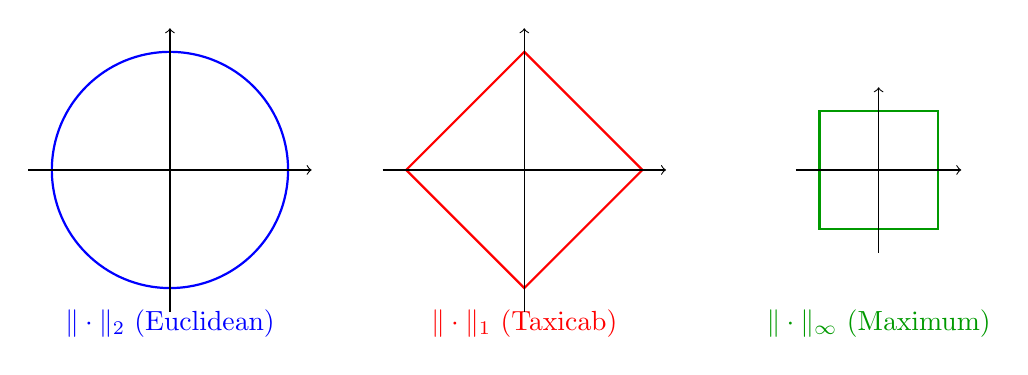
\begin{tikzpicture}[scale=1.5]
    % Unit ball for l_2 (circle)
    \draw[thick, blue] (0,0) circle (1);
    \node[blue] at (0, -1.3) {$\|\cdot\|_2$ (Euclidean)};
    
    % Unit ball for l_1 (diamond)
    \draw[thick, red] (3,1) -- (4,0) -- (3,-1) -- (2,0) -- cycle;
    \node[red] at (3, -1.3) {$\|\cdot\|_1$ (Taxicab)};
    
    % Unit ball for l_infty (square)
    \draw[thick, green!60!black] (5.5,-0.5) rectangle (6.5,0.5);
    \node[green!60!black] at (6, -1.3) {$\|\cdot\|_\infty$ (Maximum)};
    
    % Axes for reference
    \draw[->] (-1.2,0) -- (1.2,0);
    \draw[->] (0,-1.2) -- (0,1.2);
    
    \draw[->] (1.8,0) -- (4.2,0);
    \draw[->] (3,-1.2) -- (3,1.2);
    
    \draw[->] (5.3,0) -- (6.7,0);
    \draw[->] (6,-0.7) -- (6,0.7);
\end{tikzpicture}
\end{center}

\section{Distances and Open Sets}

\subsection{Defining Distance}
Given any norm $\|\cdot\|$, we define the distance between two points $x, y \in V$ as:
\[ d(x, y) = \|y - x\| \]
This definition ensures that distance is \textbf{translation invariant}: the distance between $x$ and $y$ depends only on the vector connecting them ($y-x$), not on their absolute positions.

\subsection{Open Balls and Topology}
The \textbf{open ball} of radius $r$ centered at $x$ is the set of all points strictly closer to $x$ than $r$:
\[ B(x, r) = \{ y \in \mathbb{R}^n \mid \|y - x\| < r \} \]
While the geometric \textit{shape} of these balls changes depending on the norm (circle, square, diamond), the \textit{topology} (the collection of open sets) they generate is identical in finite-dimensional spaces. 

\textbf{Remark:} The equivalence of topologies induced by different norms in finite-dimensional spaces is a consequence of the \textbf{norm equivalence theorem}, which states that any two norms on a finite-dimensional vector space are equivalent (i.e., they induce the same notions of convergence and continuity). The proof of this theorem is beyond the scope of this chapter, but it is a fundamental result in functional analysis.

\section{Inner Product Spaces and Angles}

Having established how to measure \textit{length} via norms, we now introduce a richer structure that also captures \textit{angles} between vectors. While norms tell us ``how long'' a vector is, inner products tell us ``how aligned'' two vectors are. This additional structure is essential for discussing orthogonality, projections, and geometric relationships in $\mathbb{R}^n$.

\subsection{Inner Product Definition}
An inner product generalizes the dot product. It allows us to talk about angles and orthogonality.
The standard Euclidean inner product on $\mathbb{R}^n$ is:
\[ \langle x, y \rangle = \sum_{i=1}^n x_i y_i \]

\textbf{Brief Review from Linear Algebra:} An inner product on a real vector space $V$ is a function $\langle \cdot, \cdot \rangle: V \times V \to \mathbb{R}$ satisfying:
\begin{itemize}
    \item \textbf{Symmetry:} $\langle x, y \rangle = \langle y, x \rangle$
    \item \textbf{Linearity:} $\langle \alpha x + \beta y, z \rangle = \alpha \langle x, z \rangle + \beta \langle y, z \rangle$
    \item \textbf{Positive Definiteness:} $\langle x, x \rangle \ge 0$ with equality if and only if $x = 0$
\end{itemize}

Note that $\|x\|_2 = \sqrt{\langle x, x \rangle}$, so the Euclidean norm is induced by the inner product.

\subsection{Cauchy-Schwarz Inequality}
\begin{theorem}[Cauchy-Schwarz Inequality]
For any $u, v$ in an inner product space:
\[ |\langle u, v \rangle| \le \|u\|_2 \|v\|_2 \]
where $\|x\|_2 = \sqrt{\langle x, x \rangle}$.
\end{theorem}

\begin{proof}
If $v = 0$, both sides equal zero and the inequality holds. Assume $v \ne 0$.

For any $t \in \mathbb{R}$, consider the vector $u - tv$. By positive definiteness:
\[ 0 \le \langle u - tv, u - tv \rangle \]

Expanding using linearity and symmetry:
\begin{align*}
0 &\le \langle u - tv, u - tv \rangle \\
&= \langle u, u \rangle - 2t \langle u, v \rangle + t^2 \langle v, v \rangle \\
&= \|u\|_2^2 - 2t \langle u, v \rangle + t^2 \|v\|_2^2
\end{align*}

This is a quadratic in $t$ that is always non-negative. Choose $t = \frac{\langle u, v \rangle}{\|v\|_2^2}$ to minimize the quadratic:
\begin{align*}
0 &\le \|u\|_2^2 - 2 \cdot \frac{\langle u, v \rangle}{\|v\|_2^2} \cdot \langle u, v \rangle + \left(\frac{\langle u, v \rangle}{\|v\|_2^2}\right)^2 \|v\|_2^2 \\
&= \|u\|_2^2 - \frac{2\langle u, v \rangle^2}{\|v\|_2^2} + \frac{\langle u, v \rangle^2}{\|v\|_2^2} \\
&= \|u\|_2^2 - \frac{\langle u, v \rangle^2}{\|v\|_2^2}
\end{align*}

Rearranging: $\langle u, v \rangle^2 \le \|u\|_2^2 \|v\|_2^2$. Taking square roots gives the result.
\end{proof}

\textbf{Geometric Intuition:} This inequality essentially says that $|\cos \theta| \le 1$, where $\theta$ is the angle between $u$ and $v$. Indeed, we define $\cos \theta = \frac{\langle u, v \rangle}{\|u\|_2 \|v\|_2}$, and Cauchy-Schwarz ensures this ratio is always between $-1$ and $1$.

\subsection{Worked Example: Verifying Cauchy-Schwarz}
Let $u = (1, 2, 3)$ and $v = (4, 5, 6)$ in $\mathbb{R}^3$.
\begin{align*}
\langle u, v \rangle &= 1 \cdot 4 + 2 \cdot 5 + 3 \cdot 6 = 4 + 10 + 18 = 32 \\
\|u\|_2 &= \sqrt{1^2 + 2^2 + 3^2} = \sqrt{14} \\
\|v\|_2 &= \sqrt{4^2 + 5^2 + 6^2} = \sqrt{77}
\end{align*}

Cauchy-Schwarz states: $|\langle u, v \rangle| \le \|u\|_2 \|v\|_2$

Checking: $32 \le \sqrt{14} \cdot \sqrt{77} = \sqrt{1078} \approx 32.83$ \checkmark

\subsection{Triangle Inequality Proof (for $\ell_2$)}
Using Cauchy-Schwarz, we can now complete the proof that $\|\cdot\|_2$ satisfies the triangle inequality:
\begin{proof}
\begin{align*}
\|x+y\|_2^2 &= \langle x+y, x+y \rangle \\
&= \langle x, x \rangle + 2\langle x, y \rangle + \langle y, y \rangle \\
&= \|x\|_2^2 + 2\langle x, y \rangle + \|y\|_2^2 \\
&\le \|x\|_2^2 + 2\|x\|_2\|y\|_2 + \|y\|_2^2 \quad \text{(by Cauchy-Schwarz)} \\
&= (\|x\|_2 + \|y\|_2)^2
\end{align*}
Taking the square root gives $\|x+y\|_2 \le \|x\|_2 + \|y\|_2$.
\end{proof}
\textbf{Equality Condition:} Equality holds if and only if $x$ and $y$ are non-negative scalar multiples of each other (i.e., they point in the same direction).

\section{Orthogonality and the Pythagorean Theorem}

\subsection{Definition of Orthogonality}
Two vectors $u, v \in \mathbb{R}^n$ are called \textbf{orthogonal} (denoted $u \perp v$) if their inner product is zero:
\[ u \perp v \quad \iff \quad \langle u, v \rangle = 0 \]

\textbf{Geometric Intuition:} This generalizes the notion of perpendicularity from Euclidean geometry. When two vectors are orthogonal, they form a $90^\circ$ angle. Recall that $\cos \theta = \frac{\langle u, v \rangle}{\|u\|_2 \|v\|_2}$, so $\langle u, v \rangle = 0$ means $\cos \theta = 0$, which occurs when $\theta = 90^\circ$.

\subsection{The Pythagorean Theorem}
\begin{theorem}[Pythagorean Theorem in $\mathbb{R}^n$]
If $u \perp v$, then:
\[ \|u + v\|_2^2 = \|u\|_2^2 + \|v\|_2^2 \]
\end{theorem}

\begin{proof}
\begin{align*}
\|u + v\|_2^2 &= \langle u + v, u + v \rangle \\
&= \langle u, u \rangle + 2\langle u, v \rangle + \langle v, v \rangle \\
&= \|u\|_2^2 + 2 \cdot 0 + \|v\|_2^2 \quad \text{(since $u \perp v$ means $\langle u, v \rangle = 0$)} \\
&= \|u\|_2^2 + \|v\|_2^2
\end{align*}
\end{proof}

This is the familiar Pythagorean theorem from high school geometry, but now proven rigorously in $\mathbb{R}^n$.

\subsection{Worked Example: Finding Orthogonal Vectors}
Let $u = (2, 3)$ in $\mathbb{R}^2$. Find a vector $v$ orthogonal to $u$.

We need $\langle u, v \rangle = 0$. If $v = (v_1, v_2)$, then:
\[ 2v_1 + 3v_2 = 0 \]

One solution is $v = (3, -2)$ (we can verify: $2 \cdot 3 + 3 \cdot (-2) = 6 - 6 = 0$ \checkmark).

In fact, the set of all vectors orthogonal to $u$ forms a line through the origin perpendicular to $u$. Any scalar multiple of $(3, -2)$ is also orthogonal to $u$.

\textbf{Verification of Pythagorean Theorem:}
\begin{align*}
\|u\|_2^2 &= 2^2 + 3^2 = 13 \\
\|v\|_2^2 &= 3^2 + (-2)^2 = 13 \\
\|u + v\|_2^2 &= \|(5, 1)\|_2^2 = 25 + 1 = 26 = 13 + 13 \quad \checkmark
\end{align*}

\subsection{Preview: Orthonormal Bases}
\textbf{Brief Linear Algebra Review:} An \textbf{orthonormal basis} for $\mathbb{R}^n$ is a set of $n$ vectors $\{e_1, \dots, e_n\}$ such that:
\begin{itemize}
    \item $\|e_i\|_2 = 1$ for all $i$ (normalized)
    \item $\langle e_i, e_j \rangle = 0$ for $i \ne j$ (mutually orthogonal)
\end{itemize}

The standard basis $\{(1,0,\dots,0), (0,1,0,\dots,0), \dots, (0,\dots,0,1)\}$ is an example. Orthonormal bases are particularly useful for computations and will appear in later chapters when we discuss change of coordinates and optimization.

\section{Chapter Summary}

In this chapter, we developed the tools to measure length, distance, and angles in $\mathbb{R}^n$:

\textbf{Key Definitions:}
\begin{itemize}
    \item \textbf{Norm:} A function $\|\cdot\|: V \to \mathbb{R}$ satisfying non-negativity, homogeneity, and triangle inequality
    \item \textbf{Standard Norms:} $\|x\|_1 = \sum |x_i|$, $\|x\|_2 = \sqrt{\sum x_i^2}$, $\|x\|_\infty = \max |x_i|$
    \item \textbf{Distance:} $d(x, y) = \|y - x\|$
    \item \textbf{Inner Product:} $\langle x, y \rangle = \sum x_i y_i$ (generalizes dot product)
    \item \textbf{Orthogonality:} $u \perp v \iff \langle u, v \rangle = 0$
\end{itemize}

\textbf{Key Theorems:}
\begin{itemize}
    \item \textbf{Cauchy-Schwarz:} $|\langle u, v \rangle| \le \|u\|_2 \|v\|_2$
    \item \textbf{Triangle Inequality:} $\|x+y\|_2 \le \|x\|_2 + \|y\|_2$ (proven using Cauchy-Schwarz)
    \item \textbf{Pythagorean Theorem:} $\|u+v\|_2^2 = \|u\|_2^2 + \|v\|_2^2$ when $u \perp v$
    \item \textbf{Norm Equivalence (stated):} All norms on finite-dimensional spaces induce the same topology
\end{itemize}

These concepts are essential for Chapter 3, where we will use norms to define the O notation for comparing functions in $\mathbb{R}^n$, and Chapter 4, where distances and norms enable us to define derivatives as best linear approximations.
